% Provenance (never printed): see sources/outline_sources.md (Year 2: Goldschmidt's
% classification; the chondritic Earth; core, mantle and crust compositions; trace
% elements and normalised diagrams). Curves from figdata/bachelor-2/geochem.py; exercise
% and problem values in the Book 4 scratch calculator calc/ch03.py.
\chapter{De elementen in de aarde}\label{ch:b2:elements-in-the-earth}

Een ton gesteente van de continenten bevat ongeveer anderhalve milligram
goud. Een ton van de \omterm{def:b2:planet-formation-meteorites:chondrule}{koolstofhoudende chondrieten} van het vorige hoofdstuk, de meest
primitieve stenen die uit de hemel vallen, bevat er ongeveer honderd keer meer. De
aarde werd uit zulk materiaal opgebouwd, dus het goud ontbreekt niet in de
aarde: het zit elders. Combineer de geschatte samenstellingen van de kern en van
de silicaataarde met de massa van de kern, en meer dan 99 procent van het
goud van de aarde blijkt in de kern te zitten, waar het vroeg in de geschiedenis van de aarde
met het ijzer is weggezakt. Goud hoort bij een familie van elementen die metallisch
ijzer volgen; andere volgen sulfide, weer andere het silicaatgesteente, en nog andere ontsnappen
naar de lucht. Dit hoofdstuk deelt de elementen in deze families in, gebruikt de
\omterm{def:b2:planet-formation-meteorites:chondrule}{chondrieten} om de samenstelling van de hele aarde te reconstrueren en haar
kern te wegen, beschrijft de samenstellingen van de mantel, de oceanische korst en de
continentale korst, en introduceert de \omterm{def:b2:elements-in-the-earth:trace}{sporenelementen} en de diagrammen waarop
geochemici de geschiedenis van een gesteente aflezen.
% ledger: rg03:ucc-trace, lodders:ci-table, mcd03:core, ms95:pm-trace, data:prem

\begin{recall}
De aarde heeft een metallische kern, grotendeels ijzer, onder een silicaatmantel en een dunne
korst; de seismologie geeft de straal en de dichtheid van elke laag, en de kern
is 5 tot 10 procent minder dicht dan zuiver ijzer bij dezelfde druk en
temperatuur zou zijn, wat lichte elementen in de kern vereist: silicium, zwavel, koolstof,
zuurstof en waterstof zijn de kandidaten (Boek~3). De
elektronegativiteit van een element geeft aan hoe sterk zijn atomen de
elektronen van een binding aantrekken, en de straal van een ion hangt af van zijn lading en van het
aantal buren (scheikunde, eerste jaar universiteit). Een
verdelingscoëfficiënt is de verhouding van de concentraties van een stof in twee fasen in
evenwicht (scheikunde, eerste jaar universiteit). \omterm{def:b2:planet-formation-meteorites:chondrule}{Chondrieten}, \omterm{def:b2:planet-formation-meteorites:chondrule}{koolstofhoudende
chondrieten} en de \omterm{def:b2:planet-formation-meteorites:condensation}{condensatiereeks} werden ingevoerd in
\cref{ch:b2:planet-formation-meteorites}.
\end{recall}
% ledger: badro:core

\section{De classificatie van Goldschmidt}

Wanneer een chondritisch lichaam smelt, scheidt zijn materie zich in niet-mengbare vloeistoffen: een
dicht metaal van ijzer en nikkel, een sulfidesmelt als er genoeg zwavel is, en een
silicaatsmelt, met daarboven een gasfase. Elk element verdeelt zich over
deze fasen volgens zijn chemie, en dezelfde verdeling ziet men bij het
smelten van erts, waar gesmolten ijzer, een sulfidesteen en een silicaatslak zich in de
oven scheiden.

\begin{definition}[Classificatie van Goldschmidt]
\label{def:b2:elements-in-the-earth:goldschmidt}
De \emph{classificatie van Goldschmidt}\index{classificatie van Goldschmidt} deelt
de elementen in naar de fase die ze verkiezen in een lichaam dat zich scheidt in metaal,
sulfide, silicaat en gas. Een \emph{lithofiel element}\index{lithofiel element}
verkiest silicaat en oxide; een \emph{siderofiel element}\index{siderofiel element} verkiest metallisch ijzer; een \emph{chalcofiel
element}\index{chalcofiel element} verkiest sulfide; een \emph{atmofiel
element}\index{atmofiel element} blijft in het gas, als gas of als vluchtige
verbinding.
\end{definition}

De klassen volgen de chemie van de binding. \omterm{def:b2:elements-in-the-earth:goldschmidt}{Lithofiele elementen}, zoals de
alkali- en aardalkalimetalen, aluminium, titaan of de \omterm{def:b2:elements-in-the-earth:ree}{zeldzame aarden}, staan
hun elektronen gemakkelijk af aan zuurstof, dat veel elektronegatiever is, en
vormen er ionbindingen mee. \omterm{def:b2:elements-in-the-earth:goldschmidt}{Siderofiele elementen}, de platinametalen, goud,
nikkel en kobalt, hebben een elektronegativiteit dicht bij die van ijzer, binden zwak
met zuurstof en lossen op in het metaal. \omterm{def:b2:elements-in-the-earth:goldschmidt}{Chalcofiele elementen}, waaronder koper, zink, lood,
zilver en cadmium, vormen met zwavel bindingen die meer covalent zijn.
De \omterm{def:b2:elements-in-the-earth:goldschmidt}{atmofiele elementen} zijn de edelgassen, stikstof en waterstof. Veel
elementen behoren tot twee klassen, afhankelijk van de omstandigheden: ijzer zelf is
siderofiel in een metaalrijk lichaam en lithofiel in de geoxideerde mantel, waar het
in olivijn en pyroxeen zit; wolfraam en molybdeen zijn siderofiel in de
aarde, maar een groot deel ervan is in de mantel gebleven (figuur hieronder).

\begin{omfigure}
\centering
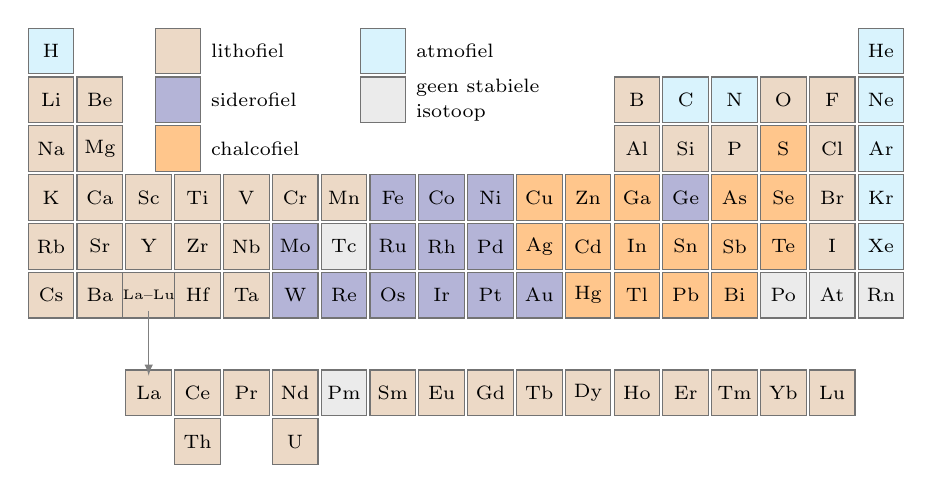
\begin{tikzpicture}[x=0.62cm, y=-0.62cm,
  lith/.style={fill=brown!30}, sid/.style={fill=blue!30!gray!45},
  chal/.style={fill=orange!45}, atm/.style={fill=cyan!15}, none/.style={fill=black!8},
  cell/.style={draw=black!55, minimum size=0.58cm, inner sep=0pt, font=\scriptsize}]
\foreach \s/\c/\r/\k in {H/1/1/atm, He/18/1/atm,
  Li/1/2/lith, Be/2/2/lith, B/13/2/lith, C/14/2/atm, N/15/2/atm, O/16/2/lith,
  F/17/2/lith, Ne/18/2/atm,
  Na/1/3/lith, Mg/2/3/lith, Al/13/3/lith, Si/14/3/lith, P/15/3/lith, S/16/3/chal,
  Cl/17/3/lith, Ar/18/3/atm,
  K/1/4/lith, Ca/2/4/lith, Sc/3/4/lith, Ti/4/4/lith, V/5/4/lith, Cr/6/4/lith,
  Mn/7/4/lith, Fe/8/4/sid, Co/9/4/sid, Ni/10/4/sid, Cu/11/4/chal, Zn/12/4/chal,
  Ga/13/4/chal, Ge/14/4/sid, As/15/4/chal, Se/16/4/chal, Br/17/4/lith, Kr/18/4/atm,
  Rb/1/5/lith, Sr/2/5/lith, Y/3/5/lith, Zr/4/5/lith, Nb/5/5/lith, Mo/6/5/sid,
  Tc/7/5/none, Ru/8/5/sid, Rh/9/5/sid, Pd/10/5/sid, Ag/11/5/chal, Cd/12/5/chal,
  In/13/5/chal, Sn/14/5/chal, Sb/15/5/chal, Te/16/5/chal, I/17/5/lith, Xe/18/5/atm,
  Cs/1/6/lith, Ba/2/6/lith, Hf/4/6/lith, Ta/5/6/lith, W/6/6/sid, Re/7/6/sid,
  Os/8/6/sid, Ir/9/6/sid, Pt/10/6/sid, Au/11/6/sid, Hg/12/6/chal, Tl/13/6/chal,
  Pb/14/6/chal, Bi/15/6/chal, Po/16/6/none, At/17/6/none, Rn/18/6/none,
  La/3/8/lith, Ce/4/8/lith, Pr/5/8/lith, Nd/6/8/lith, Pm/7/8/none, Sm/8/8/lith,
  Eu/9/8/lith, Gd/10/8/lith, Tb/11/8/lith, Dy/12/8/lith, Ho/13/8/lith,
  Er/14/8/lith, Tm/15/8/lith, Yb/16/8/lith, Lu/17/8/lith,
  Th/4/9/lith, U/6/9/lith}
  \node[cell, \k] at (\c,\r) {\s};
\node[cell, lith, minimum width=0.58cm] at (3,6) {\tiny La--Lu};
\draw[black!50, -latex] (3,6.32) -- (3,7.65);
% legend
\foreach \k/\t/\x/\y in {lith/lithofiel/3.6/1, sid/siderofiel/3.6/2,
  chal/chalcofiel/3.6/3, atm/atmofiel/7.8/1, none/{\shortstack[l]{geen stabiele\\isotoop}}/7.8/2}
  \node[cell, \k, label={[font=\scriptsize]east:\t}] at (\x,\y) {};
\end{tikzpicture}
\par\smallskip{\small De klassen van Goldschmidt van de stabiele elementen en van thorium en uranium, waarvan de langlevende isotopen bewaard zijn sinds de geboorte van de aarde, gekleurd volgens de klasse
die in de aarde overheerst; de elementen van de rij van de \omterm{def:b2:elements-in-the-earth:ree}{zeldzame aarden} staan in het vakje
La--Lu. Meerdere elementen behoren tot twee klassen: ijzer, nikkel en kobalt zijn ook
lithofiel in de geoxideerde mantel; koolstof is ook siderofiel, fosfor
siderofiel in \omterm{def:b2:planet-formation-meteorites:fall-find}{meteorieten}.}
\end{omfigure}

\section{De chondritische aarde}

Niemand kan de aarde als geheel bemonsteren: de kern is onbereikbaar, en de
mantel bereikt het oppervlak alleen in brokstukken. De samenstelling van de aarde als geheel wordt
in plaats daarvan opgebouwd uit twee soorten aanwijzingen: de \omterm{def:b2:planet-formation-meteorites:fall-find}{meteorieten}, die het
materiaal bemonsteren waaruit de planeten ontstonden, en de gesteenten van de mantel en de
smelten die eruit voortkomen.

\begin{definition}[CI-chondriet]\label{def:b2:elements-in-the-earth:ci}
Een \emph{CI-chondriet}\index{CI-chondriet} is een lid van de groep
\omterm{def:b2:planet-formation-meteorites:chondrule}{koolstofhoudende chondrieten} die genoemd is naar de \omterm{def:b2:planet-formation-meteorites:fall-find}{meteoriet} van Ivuna: zwarte, brokkelige stenen
die bijna geheel uit fijnkorrelige matrix bestaan, rijk aan waterhoudende mineralen en
koolstof, bijna zonder \omterm{def:b2:planet-formation-meteorites:chondrule}{chondrulen}. Op waterstof, koolstof, stikstof, zuurstof en de
edelgassen na is hun samenstelling van alle bekende materialen die welke het dichtst bij die van
de fotosfeer van de Zon ligt; ze vormen de referentiesamenstelling van de geochemie.
\end{definition}

De groep telt vijf \omterm{def:b2:planet-formation-meteorites:fall-find}{meteorieten}, allemaal vallen: Alais (1806), Orgueil
(1864), Tonk (1911), Ivuna (1938) en Revelstoke (1965); Orgueil is de grootste,
met veertien kilogram. De samenstelling die voor de groep wordt aangenomen, is een gewogen gemiddelde
van hun analyses, element per element; de waarden die in dit hoofdstuk worden gebruikt, worden
vermeld waar ze nodig zijn.
% ledger: lodders:ci-table

\begin{definition}[Refractaire en vluchtige elementen]
\label{def:b2:elements-in-the-earth:volatility}
Een \emph{refractair element}\index{refractair element} is een element waarvan de
50-procent-condensatietemperatuur (\cref{ch:b2:planet-formation-meteorites}) boven
die van magnesium, silicium en ijzer ligt, \qtyrange{1310}{1340}{K} bij
\qty{e-4}{bar}; een
\emph{vluchtig element}\index{vluchtig element} is een element waarvan de
\omterm{def:b2:planet-formation-meteorites:condensation}{condensatietemperatuur} eronder ligt.
\end{definition}

Het magnesiumgehalte dient als maatstaf. Magnesium is lithofiel, condenseert
met het grootste deel van het gesteente en gaat niet in de kern, dus de verhouding van een element
tot magnesium in de silicaataarde, gedeeld door dezelfde verhouding in \omterm{def:b2:elements-in-the-earth:ci}{CI-chondrieten},
meet hoeveel van dat element de silicaataarde heeft behouden ten opzichte van een
chondritisch uitgangsmateriaal. Het water, de koolstof en de andere vluchtige verbindingen die
\omterm{def:b2:elements-in-the-earth:ci}{CI-chondrieten} bevatten en die de aarde niet heeft behouden, vallen uit de verhouding weg.

\begin{definition}[Totale silicaataarde, primitieve mantel]
\label{def:b2:elements-in-the-earth:bse}
De \emph{totale silicaataarde}\index{totale silicaataarde} is de aarde zonder
haar kern: mantel, korst, oceaan en dampkring samen genomen, zoals ze zouden zijn als ze
gemengd waren. Dezelfde samenstelling heet de \emph{primitieve mantel}\index{primitieve mantel}: de mantel zoals hij was nadat de kern zich had gevormd en voordat er korst
aan was onttrokken.
\end{definition}

Schattingen van de \omterm{def:b2:elements-in-the-earth:bse}{primitieve mantel} steunen op de mantelgesteenten die het
minst smelt hebben verloren, peridotieten die als xenolieten in lava's naar boven zijn gebracht (foto hieronder) of
in gebergtegordels dagzomen, en op de aanname dat de refractaire \omterm{def:b2:elements-in-the-earth:goldschmidt}{lithofiele
elementen} onderling in chondritische verhoudingen staan. Een veelgebruikt resultaat, met
22.8 procent magnesium, 21.0 procent silicium en 6.26 procent ijzer in massa, staat in de
tabel van samenstellingen verderop.
% ledger: ms95:pm-trace, ms95:pm-oxides

\begin{omfigure}
\centering
\begin{minipage}{0.48\linewidth}
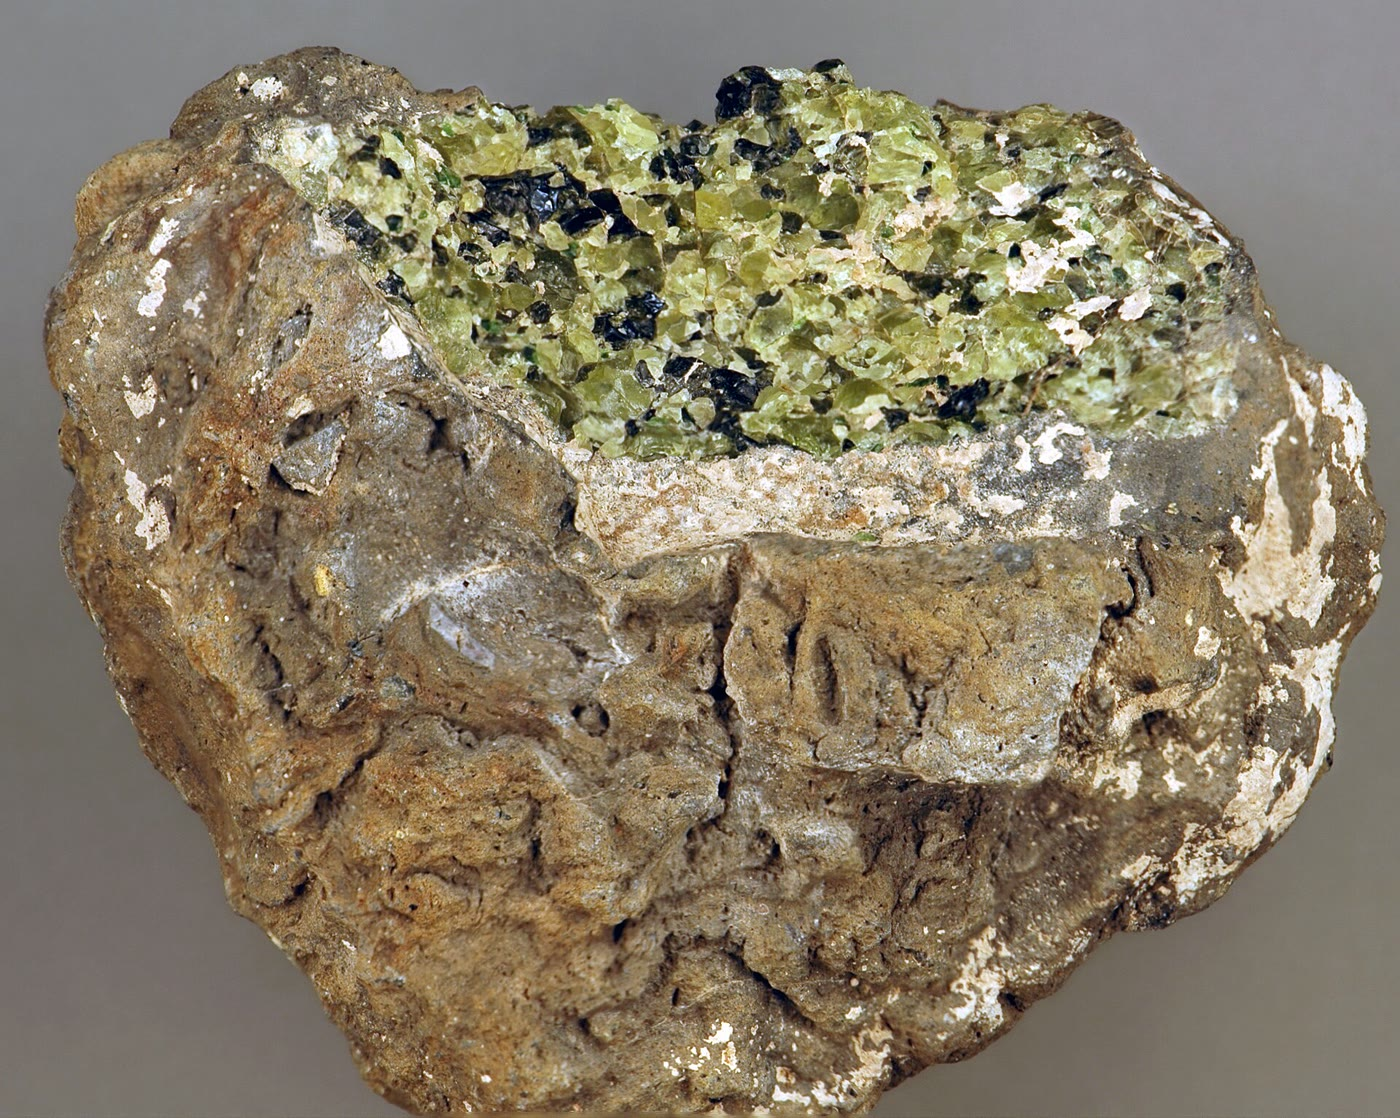
\includegraphics[width=\linewidth]{images/book4/b2-lherzolite-xenolith.jpg}
\end{minipage}\hfill
\begin{minipage}{0.48\linewidth}
{\small Een nodule van mantelperidotiet (lherzoliet) in een basaltlava van
Kilbourne Hole, New Mexico, op zijn breedst \qty{7.4}{cm}: geelgroen
olivijn met donker pyroxeen. De lava rukte hem los uit de bovenmantel en voerde
hem naar het oppervlak. James St.~John, CC BY 2.0.}
\end{minipage}
\end{omfigure}

De figuur hieronder vergelijkt deze silicaataarde met \omterm{def:b2:elements-in-the-earth:ci}{CI-chondrieten}, element per
element, tegen de \omterm{def:b2:planet-formation-meteorites:condensation}{condensatietemperatuur} van het vorige hoofdstuk. Ze rangschikt
de elementen op een manier die geen ander bewijs kan evenaren. De refractaire \omterm{def:b2:elements-in-the-earth:goldschmidt}{lithofiele
elementen}, van zirkonium en de \omterm{def:b2:elements-in-the-earth:ree}{zeldzame aarden} tot strontium en barium, staan
alle op hetzelfde niveau, op twintig procent na: de silicaataarde
heeft ze alle in hun chondritische verhoudingen behouden. De vluchtige \omterm{def:b2:elements-in-the-earth:goldschmidt}{lithofiele elementen}
lopen terug met hun \omterm{def:b2:planet-formation-meteorites:condensation}{condensatietemperatuur}: ongeveer een vijfde van het kalium
en het natrium, een tiende van het rubidium, een honderdste van het chloor en enkele
duizendsten van het broom en het jodium zijn aanwezig. De \omterm{def:b2:elements-in-the-earth:goldschmidt}{siderofiele elementen} liggen ver onder elk \omterm{def:b2:elements-in-the-earth:goldschmidt}{lithofiel element}
met dezelfde vluchtigheid: de silicaataarde bevat een zevende van haar aandeel aan
ijzer, een dertiende van het nikkel, en ongeveer drie duizendsten van de
platinametalen en het goud. Die gingen naar de kern. De \omterm{def:b2:elements-in-the-earth:goldschmidt}{chalcofiele
elementen}, die meestal ook vluchtig zijn, zijn op beide gronden verarmd.

\begin{omfigure}
\centering
\begin{tikzpicture}
\begin{axis}[omrecord, width=0.95\linewidth, height=8.2cm, ymode=log,
  xmin=500, xmax=1800, ymin=8e-4, ymax=3, x dir=reverse,
  xlabel={50-procent-condensatietemperatuur bij \qty{e-4}{bar} (K)},
  ylabel={$(X/\mathrm{Mg})_{\mathrm{BSE}}\,/\,(X/\mathrm{Mg})_{\mathrm{CI}}$},
  legend pos=south west, legend cell align=left, legend style={font=\scriptsize},
  tick label style={font=\scriptsize}, label style={font=\small},
  scaled x ticks=false, xticklabel style={/pgf/number format/1000 sep={}}]
\addplot[black!40, dashed, domain=500:1800, samples=2, forget plot] {1};
\addplot[only marks, mark=*, mark size=1.6pt, brown!70!black]
  table[x=T, y=ratio] {figdata/out/bachelor-2-geochem-volat-lith.dat};
\addlegendentry{lithofiel}
\addplot[only marks, mark=square*, mark size=1.6pt, blue!60!black]
  table[x=T, y=ratio] {figdata/out/bachelor-2-geochem-volat-sid.dat};
\addlegendentry{siderofiel}
\addplot[only marks, mark=triangle*, mark size=2pt, orange!80!black]
  table[x=T, y=ratio] {figdata/out/bachelor-2-geochem-volat-chal.dat};
\addlegendentry{chalcofiel}
\node[font=\tiny, brown!50!black, anchor=south] at (axis cs:1600,1.35)
  {Zr, Hf, Al, Sc, Y, Th, U, Ti, Ca, Sr, Ba, zeldzame aarden};
\begin{scope}[font=\tiny, brown!50!black]
\node[anchor=west] at (axis cs:1328,1.0) {Mg};
\node[anchor=north] at (axis cs:1310,0.80) {Si};
\node[anchor=west] at (axis cs:1150,0.23) {Mn};
\node[anchor=south] at (axis cs:1142,0.47) {Li};
\node[anchor=south] at (axis cs:1010,0.195) {K};
\node[anchor=north] at (axis cs:958,0.22) {Na};
\node[anchor=north] at (axis cs:908,0.175) {B};
\node[anchor=north] at (axis cs:800,0.116) {Rb};
\node[anchor=south] at (axis cs:734,0.175) {F};
\node[anchor=west] at (axis cs:795,0.0477) {Cs};
\node[anchor=west] at (axis cs:944,0.0102) {Cl};
\node[anchor=north] at (axis cs:546,0.0061) {Br};
\node[anchor=south] at (axis cs:535,0.0088) {I};
\end{scope}
\begin{scope}[font=\tiny, blue!50!black]
\node[anchor=west] at (axis cs:1325,0.144) {Fe};
\node[anchor=east] at (axis cs:1364,0.0775) {Ni};
\node[anchor=west] at (axis cs:1342,0.088) {Co};
\node[anchor=west] at (axis cs:1780,0.137) {W};
\node[anchor=south] at (axis cs:1590,0.0206) {Mo};
\node[anchor=north] at (axis cs:883,0.0139) {Ge};
\node[anchor=north] at (axis cs:1500,0.0026) {Re, Os, Ir, Ru, Pt, Pd};
\node[anchor=north] at (axis cs:1060,0.0026) {Au};
\end{scope}
\begin{scope}[font=\tiny, orange!60!black]
\node[anchor=west] at (axis cs:1030,0.0993) {Cu};
\node[anchor=north] at (axis cs:996,0.0167) {Ag};
\node[anchor=south] at (axis cs:726,0.0746) {Zn};
\node[anchor=south] at (axis cs:704,0.0325) {Sn};
\node[anchor=east] at (axis cs:735,0.0246) {Pb};
\node[anchor=west] at (axis cs:648,0.0249) {Cd};
\node[anchor=east] at (axis cs:715,0.0022) {Te};
\node[anchor=north] at (axis cs:690,0.0016) {Se};
\node[anchor=west] at (axis cs:660,0.0019) {S};
\end{scope}
\end{axis}
\end{tikzpicture}
\par\smallskip{\small De silicaataarde vergeleken met \omterm{def:b2:elements-in-the-earth:ci}{CI-chondrieten}: voor elk element $X$ de
verhouding $X/\mathrm{Mg}$ in de \omterm{def:b2:elements-in-the-earth:bse}{totale silicaataarde} gedeeld door dezelfde verhouding in
\omterm{def:b2:elements-in-the-earth:ci}{CI-chondrieten}, tegen de 50-procent-condensatietemperatuur (heet links).
Refractaire \omterm{def:b2:elements-in-the-earth:goldschmidt}{lithofiele elementen} zijn onderling chondritisch; vluchtige
zijn verarmd naarmate de \omterm{def:b2:planet-formation-meteorites:condensation}{condensatietemperatuur} daalt; siderofiele en
\omterm{def:b2:elements-in-the-earth:goldschmidt}{chalcofiele elementen} zijn veel sterker verarmd. Gegevens: McDonough en Sun (1995);
Lodders (2003).}
\end{omfigure}
% ledger: ms95:pm-trace, lodders:ci-table, lodders:tc-table, lodders:tc-more

De refractaire \omterm{def:b2:elements-in-the-earth:goldschmidt}{lithofiele elementen} staan ongeveer 15 procent boven magnesium. De
twee kunnen niet allebei precies chondritisch zijn: ofwel heeft de aarde \omterm{def:b2:elements-in-the-earth:volatility}{refractaire
elementen} gewonnen, ofwel heeft ze wat magnesium verloren, ofwel is het magnesium van het model een
onderschatting (\cref{exo:b2:elements-in-the-earth:12}). Silicium, op 0.83, blijft verder onder het
refractaire niveau; een deel van het ontbrekende silicium zit misschien in de kern (probleem).

De \omterm{def:b2:elements-in-the-earth:goldschmidt}{siderofiele elementen} in de silicaataarde, gecombineerd met een chondritische aarde als
geheel, wegen de kern. Stel dat de aarde als geheel de CI-verhouding $r_X = X/\mathrm{Mg}$ heeft
voor een \omterm{def:b2:elements-in-the-earth:goldschmidt}{siderofiel element} $X$, en dat de kern er de concentratie $c_X$ van bevat,
maar geen magnesium.

\begin{proposition}[Massafractie van de kern uit een chondritische verhouding]
\label{prop:b2:elements-in-the-earth:core}
Zij $x$ de massafractie van de kern, $C_X$ en $C_{\mathrm{Mg}}$ de
concentraties van $X$ en magnesium in de silicaataarde, en $c_X$ die van $X$ in
de kern. Als de aarde de chondritische verhouding $r_X$ heeft, dan is
\[
  \frac{x}{1-x} = \frac{r_X C_{\mathrm{Mg}} - C_X}{c_X}.
\]
\end{proposition}

\begin{proof}
Een massa $M$ aarde bevat $(1-x)MC_X + xMc_X$ aan $X$ en $(1-x)MC_{\mathrm{Mg}}$ aan
magnesium. Hun verhouding is $r_X$:
$(1-x)C_X + xc_X = r_X(1-x)C_{\mathrm{Mg}}$. Delen door $(1-x)c_X$ geeft het
resultaat.
\end{proof}

Met ijzer, $r_{\mathrm{Fe}} = \num{182800}/\num{95870} = 1.907$ in \omterm{def:b2:elements-in-the-earth:ci}{CI-chondrieten},
22.8 procent magnesium en 6.26 procent ijzer in de silicaataarde, en 85.5
procent ijzer in een modelkern, geeft de propositie $x/(1-x) = 0.435$, een kern van 30
procent van de massa van de aarde. De seismologie, die de dichtheid van het
referentiemodel van de aarde integreert, geeft 32.5 procent. De overeenstemming op een tiende na
ondersteunt het beeld van een chondritische aarde waarvan het ijzer grotendeels in de kern zit; het
verschil meet hoe ver de ijzer-magnesiumverhouding van de aarde afwijkt van de
chondritische (probleem). Dezelfde balans vertelt waar elk element van de aarde zit
(figuur hieronder): bijna al haar platina, iridium en goud, en het grootste deel van haar ijzer,
nikkel en zwavel, zitten in de kern.
% ledger: lodders:ci-table, ms95:pm-trace, mcd03:core, data:prem

\begin{omfigure}
\centering
\begin{tikzpicture}
\begin{axis}[omrecord, xbar, width=0.8\linewidth, height=6.4cm, bar width=5pt,
  xmin=0, xmax=100, ymin=0.4, ymax=14.6, y dir=reverse,
  ytick={1,...,14}, yticklabels from table={figdata/out/bachelor-2-geochem-budget.dat}{el},
  xlabel={aandeel van de voorraad van de aarde dat in de kern zit (procent)},
  tick label style={font=\scriptsize}, label style={font=\small},
  nodes near coords, nodes near coords align={horizontal},
  every node near coord/.append style={font=\tiny, /pgf/number format/fixed,
    /pgf/number format/precision=1}]
\addplot[fill=blue!35!gray!50, draw=black!60]
  table[x=share, y=idx] {figdata/out/bachelor-2-geochem-budget.dat};
\end{axis}
\end{tikzpicture}
\par\smallskip{\small Waar de elementen van de aarde zitten: het aandeel van elk element dat in
de kern zit, op basis van een modelsamenstelling van de kern, de \omterm{def:b2:elements-in-the-earth:bse}{primitieve mantel} en een kern van 32.5
procent van de massa van de aarde. Gegevens: McDonough (2003); McDonough en Sun (1995);
referentiemodel van de aarde.}
\end{omfigure}
% ledger: mcd03:core, ms95:pm-trace, data:prem

\section{Mantel en korsten}

De silicaataarde is sinds haar vorming verdeeld in een mantel en twee
soorten korst. De oceanische korst ontstaat door smelten van de mantel onder de
mid-oceanische ruggen; de continentale korst door een lange geschiedenis van smelten boven
subductiezones, herbewerking en erosie (latere hoofdstukken). Twee referentiesmelten
van de mantel verankeren de bespreking.

\begin{definition}[Basalt van mid-oceanische ruggen, oceaaneilandbasalt]
\label{def:b2:elements-in-the-earth:morb-oib}
Een \emph{basalt van mid-oceanische ruggen}\index{basalt van mid-oceanische ruggen} (MORB) is een basalt
dat bij een mid-oceanische rug is uitgevloeid, het gesteente van de top van de oceanische korst. Een
\emph{oceaaneilandbasalt}\index{oceaaneilandbasalt} (OIB) is een basalt dat is uitgevloeid
bij een oceanische vulkaan ver van plaatgrenzen, zoals die van Hawaï,
en dat gewoonlijk wordt toegeschreven aan een mantelpluim (Boek~3).
\end{definition}

De gemiddelde MORB in de tabel hieronder is een wereldwijd gemiddelde opgebouwd uit 771
rugsegmenten, waarbij elk segment gewogen is naar zijn lengte en zijn spreidingssnelheid, zodat het
gemiddelde de korst voorstelt die de ruggen produceren. De
OIB-kolom is één enkel gesteente: het basaltreferentiemateriaal BHVO-2, in 1995 genomen
uit een lava die in 1919 over de rand van de Halemaumau-krater van Kilauea, Hawaï, stroomde,
en door veel laboratoria geanalyseerd, zodat de meeste van zijn \omterm{def:b2:elements-in-the-earth:ree}{zeldzame aarden} tot op
ongeveer één procent bekend zijn. De bovenste continentale korst is een gemiddelde dat is geschat uit
oppervlaktegesteenten en sedimenten.
% ledger: gale13:allmorb, usgs:bhvo2-origin, usgs:bhvo2-major, rg14:crust

\begin{table}[h]
\centering
\small
\begin{tabular}{lrrrr}
\hline
oxide (gew.\,\%) & \omterm{def:b2:elements-in-the-earth:bse}{primitieve mantel} & MORB & OIB (BHVO-2) & bovenste cont.\ korst\\
\hline
\ce{SiO2} & 45.0 & 50.47 & 49.60 & 66.6\\
\ce{TiO2} & 0.201 & 1.68 & 2.731 & 0.64\\
\ce{Al2O3} & 4.45 & 14.70 & 13.44 & 15.4\\
FeO (totaal) & 8.05 & 10.43 & 11.15 & 5.04\\
MnO & 0.135 & 0.184 & 0.1690 & 0.10\\
MgO & 37.8 & 7.58 & 7.257 & 2.48\\
CaO & 3.55 & 11.39 & 11.40 & 3.59\\
\ce{Na2O} & 0.36 & 2.79 & 2.219 & 3.27\\
\ce{K2O} & 0.029 & 0.160 & 0.5130 & 2.80\\
\ce{P2O5} & 0.021 & 0.184 & 0.2685 & 0.15\\
\hline
\end{tabular}
\caption{Samenstelling aan hoofdelementen van vier reservoirs. BHVO-2 geeft zijn ijzer als
\ce{Fe2O3} (12.39 procent), hier omgerekend naar FeO. Gegevens: McDonough en Sun
(1995); Gale en anderen (2013); USGS-informatieblad voor BHVO-2; Rudnick en
Gao (2014).}
\label{tab:b2:elements-in-the-earth:majors}
\end{table}
% ledger: ms95:pm-oxides, gale13:allmorb, usgs:bhvo2-major, rg14:crust

Van links naar rechts gelezen vertelt de tabel het verhaal van het smelten. De mantel is een magnesiumrijke
peridotiet, met bijna 38 procent MgO en minder dan 5 procent \ce{Al2O3} en CaO.
Zijn smelten, de basalten, bevatten vijf keer minder magnesium en drie keer meer
calcium en aluminium: de elementen die gemakkelijk in de smelt gaan, verlaten de mantel
als eerste. Kalium, natrium en titaan zijn in de smelten nog rijker vergeleken
met de mantel, en kalium is het rijkst van alle in de continentale korst,
bijna honderd keer zijn concentratie in de \omterm{def:b2:elements-in-the-earth:bse}{primitieve mantel}. Silicium neemt
van de mantel naar de basalten maar weinig toe, en veel meer in de continentale
korst, waarvan het gemiddelde dicht bij dat van een granodioriet ligt.

\section{Sporenelementen}

Tien oxiden maken ongeveer 99 procent uit van elk gesteente van de tabel hierboven. De overige elementen,
aanwezig in delen per miljoen, volgen dezelfde processen als de hoofdelementen, maar
ze zijn er veel gevoeliger voor.

\begin{definition}[Sporenelement]\label{def:b2:elements-in-the-earth:trace}
Een \emph{sporenelement}\index{sporenelement} van een gesteente is een element waarvan de
concentratie volgens afspraak onder 0.1 procent in massa ligt (\qty{1000}{ppm}).
Sporenelementen vormen zelden eigen mineralen; ze vervangen hoofdelementen
op de plaatsen van de kristalroosters.
\end{definition}

Een \omterm{def:b2:elements-in-the-earth:trace}{sporenelement} is zo verdund dat zijn eigen concentratie de kristallen of de smelt
niet verandert: zijn verdeling tussen beide is dan een eenvoudige verhouding,
die over een groot bereik onafhankelijk is van zijn concentratie.

\begin{definition}[Verdelingscoëfficiënt mineraal--smelt; compatibele en
incompatibele elementen]\label{def:b2:elements-in-the-earth:partition}
De \emph{verdelingscoëfficiënt mineraal--smelt}\index{verdelingscoëfficiënt mineraal--smelt}
van een element in een mineraal is de verhouding van zijn concentraties in het
mineraal en in een silicaatsmelt die ermee in evenwicht is,
$D = C_{\mathrm{mineral}}/C_{\mathrm{melt}}$. Voor een gesteente uit meerdere mineralen met
massafracties $x_i$ is de \emph{globale verdelingscoëfficiënt}
$\bar D = C_{\mathrm{rock}}/C_{\mathrm{melt}}$. Een element is een
\emph{compatibel element}\index{compatibel element} in een gesteente als $\bar D > 1$,
een \emph{incompatibel element}\index{incompatibel element} als $\bar D < 1$.
\end{definition}

\begin{proposition}[Globale verdelingscoëfficiënt]
\label{prop:b2:elements-in-the-earth:bulk-d}
Als elk mineraal van het gesteente in evenwicht is met dezelfde smelt, is de globale
verdelingscoëfficiënt het gemiddelde van de coëfficiënten van de mineralen, gewogen naar
de massafracties: $\bar D = \sum_i x_i D_i$.
\end{proposition}

\begin{proof}
Het gesteente bevat $C_{\mathrm{rock}} = \sum_i x_i C_i$, en voor elk mineraal geldt
$C_i = D_i C_{\mathrm{melt}}$. Delen door $C_{\mathrm{melt}}$ geeft het resultaat.
\end{proof}

Of een ion in een plaats past, hangt af van zijn straal en zijn lading. Een ion dat in
straal en lading dicht bij het hoofdion van een plaats ligt, zoals \ce{Ni^2+} voor \ce{Mg^2+} in
olivijn, wordt gemakkelijk opgenomen en is compatibel. Een veel groter ion, zoals
\ce{Rb+} of \ce{Ba^2+}, of een sterker geladen ion, zoals \ce{Zr^4+} of
\ce{Nb^5+}, vervormt het rooster en wordt in de smelt uitgestoten: het is
incompatibel in de mineralen van de mantel. Twee groepen \omterm{def:b2:elements-in-the-earth:partition}{incompatibele elementen}
gedragen zich later verschillend, wanneer er water in het spel is.

\begin{definition}[Groot-ion-lithofiele elementen en elementen met hoge veldsterkte]
\label{def:b2:elements-in-the-earth:lile-hfse}
De \emph{groot-ion-lithofiele elementen}\index{groot-ion-lithofiel element}
(LILE) zijn \omterm{def:b2:elements-in-the-earth:partition}{incompatibele elementen} met grote ionen van lage lading, $+1$ of $+2$:
kalium, rubidium, cesium, strontium, barium. De
\emph{elementen met hoge veldsterkte}\index{element met hoge veldsterkte} (HFSE)
zijn \omterm{def:b2:elements-in-the-earth:partition}{incompatibele elementen} met kleine, sterk geladen ionen, $+4$ of $+5$:
zirkonium, hafnium, niobium, tantaal, titaan.
\end{definition}

De LILE lossen gemakkelijk op in waterrijke fluïda, de HFSE nauwelijks. Een gesteente
dat door water is veranderd, of een smelt die fluïda heeft geërfd, zoals boven subductiezones,
draagt daarom LILE met weinig HFSE.

\begin{definition}[Zeldzame aarden]\label{def:b2:elements-in-the-earth:ree}
De \emph{zeldzame aarden}\index{zeldzame aarde} (REE) zijn de vijftien
lanthaniden, van lanthaan tot lutetium; promethium heeft geen stabiele isotoop. Alle
zijn lithofiel en refractair, bijna alle driewaardig, en hun ionstraal
neemt regelmatig af van lanthaan tot lutetium; europium kan in gereduceerde smelten
ook tweewaardig zijn.
\end{definition}

Omdat de \omterm{def:b2:elements-in-the-earth:ree}{zeldzame aarden} geleidelijk in straal verschillen en in niets anders,
fractioneren ze geleidelijk: de lichte, lanthaan tot samarium, zijn het minst
compatibel; de zware, gadolinium tot lutetium, passen beter in sommige
mineralen, vooral granaat (figuur hieronder). In een gesteente met granaat worden de zware \omterm{def:b2:elements-in-the-earth:ree}{zeldzame
aarden} compatibel: een smelt van zo'n gesteente is rijk aan lichte \omterm{def:b2:elements-in-the-earth:ree}{zeldzame aarden} en
arm aan zware.

\begin{omfigure}
\centering
\begin{tikzpicture}
\begin{axis}[omrecord, width=0.78\linewidth, height=6.4cm, ymode=log,
  xmin=0.6, xmax=9.4, ymin=5e-4, ymax=20,
  xtick={1,...,9}, xticklabels from table={figdata/out/bachelor-2-geochem-dvals.dat}{el},
  ylabel={verdelingscoëfficiënt $D$}, legend pos=south east,
  legend cell align=left, legend style={font=\scriptsize},
  tick label style={font=\scriptsize}, label style={font=\small}]
\addplot[black!40, dashed, domain=0.6:9.4, samples=2, forget plot] {1};
\addplot[thick, green!45!black, mark=*] table[x=idx, y=cpx] {figdata/out/bachelor-2-geochem-dvals.dat};
\addlegendentry{clinopyroxeen}
\addplot[thick, red!70!black, mark=square*] table[x=idx, y=gar] {figdata/out/bachelor-2-geochem-dvals.dat};
\addlegendentry{granaat}
\addplot[thick, olive!70!black, mark=triangle*] table[x=idx, y=ol] {figdata/out/bachelor-2-geochem-dvals.dat};
\addlegendentry{olivijn + orthopyroxeen + spinel}
\addplot[very thick, black, mark=diamond*] table[x=idx, y=bulk] {figdata/out/bachelor-2-geochem-dvals.dat};
\addlegendentry{globaal gesteente (65/18/17 procent)}
\node[font=\scriptsize, anchor=south west] at (axis cs:0.7,1) {compatibel};
\node[font=\scriptsize, anchor=north west] at (axis cs:0.7,1) {incompatibel};
\end{axis}
\end{tikzpicture}
\par\smallskip{\small Verdelingscoëfficiënten mineraal--smelt van de \omterm{def:b2:elements-in-the-earth:ree}{zeldzame aarden} voor
clinopyroxeen, granaat en een mengsel van olivijn, orthopyroxeen en spinel, en de
globale coëfficiënt van een granaatpyroxeniet van 65 procent clinopyroxeen, 18
procent granaat en 17 procent van de andere mineralen (propositie hierboven). Granaat
maakt de zware \omterm{def:b2:elements-in-the-earth:ree}{zeldzame aarden} compatibel. Gegevens: Budahn (1991).}
\end{omfigure}
% ledger: budahn91:d-ree, budahn91:modes

\section{Genormaliseerde diagrammen}

De abundanties van naburige elementen verschillen met grote factoren door de
kerngeschiedenis van de materie: elementen met een even atoomnummer zijn overvloediger dan
hun oneven buren, zoals de CI-kolom van de \omterm{def:b2:elements-in-the-earth:ree}{zeldzame aarden} laat zien (lanthaan 0.232,
cerium 0.621, praseodymium 0.0928 ppm). Onbewerkt uitgezet vormen de \omterm{def:b2:elements-in-the-earth:ree}{zeldzame aarden} van een gesteente een
zaagtand die zijn geologische geschiedenis verbergt. Delen door een referentie neemt die weg.
% ledger: lodders:ci-table

\begin{definition}[Genormaliseerd diagram]\label{def:b2:elements-in-the-earth:normalised}
Een \emph{genormaliseerd diagram}\index{genormaliseerd diagram} zet voor een reeks
elementen in een vaste volgorde de concentratie in een monster gedeeld door die in een
referentie, $X_N = C_X/C_X^{\mathrm{ref}}$, uit op een logaritmische schaal. De \omterm{def:b2:elements-in-the-earth:ree}{zeldzame aarden}
worden genormaliseerd op \omterm{def:b2:elements-in-the-earth:ci}{CI-chondrieten} in de volgorde van het atoomnummer; een langere reeks
\omterm{def:b2:elements-in-the-earth:partition}{incompatibele elementen}, vaak spindiagram genoemd, wordt genormaliseerd op de
\omterm{def:b2:elements-in-the-earth:bse}{primitieve mantel} en gerangschikt naar afnemende incompatibiliteit bij het smelten van de mantel.
\end{definition}

Een monster met dezelfde verhoudingen als de referentie geeft een horizontale lijn;
de hoogte ervan geeft de verrijking. Een helling wijst op een fractionering tussen lichte en
zware elementen, gemeten met een verhouding zoals $(\mathrm{La}/\mathrm{Yb})_N$. Eén
enkel element buiten de lijn is een anomalie.

\begin{proposition}[Europiumanomalie]\label{prop:b2:elements-in-the-earth:normalised}
Op een \omterm{def:b2:elements-in-the-earth:normalised}{genormaliseerd diagram} waar het patroon een rechte lijn is in
$\log X_N$ tussen samarium en gadolinium, is de verwachte waarde voor europium, dat
midden ertussen ligt, $\mathrm{Eu}^* = \sqrt{\mathrm{Sm}_N\,\mathrm{Gd}_N}$. De
\emph{europiumanomalie}\index{europiumanomalie} is
$\mathrm{Eu}/\mathrm{Eu}^* = \mathrm{Eu}_N/\sqrt{\mathrm{Sm}_N\,\mathrm{Gd}_N}$:
onder 1 is ze negatief, boven 1 positief.
\end{proposition}

\begin{proof}
Samarium, europium en gadolinium volgen elkaar met gelijke stappen langs de as op.
Een rechte lijn in $\log X_N$ neemt in het middelste punt het gemiddelde van de eindwaarden aan:
$\log \mathrm{Eu}^* = \tfrac12(\log \mathrm{Sm}_N + \log \mathrm{Gd}_N)$, de
logaritme van het meetkundig gemiddelde.
\end{proof}

Europium is de enige \omterm{def:b2:elements-in-the-earth:ree}{zeldzame aarde} die tweewaardig kan zijn. \ce{Eu^2+} heeft bijna de
straal van \ce{Ca^2+} en \ce{Sr^2+}, dus plagioklaasveldspaat neemt het op waar het
de driewaardige \omterm{def:b2:elements-in-the-earth:ree}{zeldzame aarden} weert. Een smelt waaruit plagioklaas is gekristalliseerd,
heeft een negatieve anomalie; het achtergebleven plagioklaasrijke gesteente een positieve.

\begin{omfigure}
\centering
\begin{tikzpicture}
\begin{axis}[omrecord, width=0.8\linewidth, height=6.4cm, ymode=log,
  xmin=0.6, xmax=13.4, ymin=5, ymax=250,
  xtick={1,...,13}, xticklabels from table={figdata/out/bachelor-2-geochem-ree.dat}{el},
  ylabel={monster / CI-chondriet}, legend pos=north east, legend cell align=left,
  legend style={font=\scriptsize}, tick label style={font=\scriptsize},
  label style={font=\small}]
\addplot[thick, blue!70!black, mark=*] table[x=idx, y=morb] {figdata/out/bachelor-2-geochem-ree.dat};
\addlegendentry{gemiddelde MORB}
\addplot[thick, red!70!black, mark=square*] table[x=idx, y=oib] {figdata/out/bachelor-2-geochem-ree.dat};
\addlegendentry{OIB (BHVO-2, Hawaï)}
\addplot[thick, brown!70!black, mark=triangle*] table[x=idx, y=ucc] {figdata/out/bachelor-2-geochem-ree.dat};
\addlegendentry{bovenste continentale korst}
\end{axis}
\end{tikzpicture}
\par\smallskip{\small Patronen van de \omterm{def:b2:elements-in-the-earth:ree}{zeldzame aarden}, genormaliseerd op \omterm{def:b2:elements-in-the-earth:ci}{CI-chondrieten} (thulium weggelaten, bij
gebrek aan een MORB-waarde). De gemiddelde MORB is vlak, iets armer aan de lichte \omterm{def:b2:elements-in-the-earth:ree}{zeldzame
aarden}; het Hawaïaanse basalt is erin verrijkt; de bovenste korst is er sterk in
verrijkt, met een negatieve \omterm{prop:b2:elements-in-the-earth:normalised}{europiumanomalie}. Gegevens: Gale en anderen
(2013); USGS-blad BHVO-2; Rudnick en Gao; Lodders (2003).}
\end{omfigure}
% ledger: gale13:allmorb, usgs:bhvo2-trace, rg03:ucc-trace, lodders:ci-table

De drie patronen van de figuur hierboven lezen als drie geschiedenissen. De gemiddelde MORB
ligt ongeveer 25 keer boven \omterm{def:b2:planet-formation-meteorites:chondrule}{chondriet}, bijna vlak, met $(\mathrm{La}/\mathrm{Sm})_N
= 0.85$: zijn mantelbron had al een deel van zijn meest \omterm{def:b2:elements-in-the-earth:partition}{incompatibele elementen} afgestaan
aan vroegere smelten, waaronder de continentale korst. Het Hawaïaanse basalt is
verrijkt in de lichte \omterm{def:b2:elements-in-the-earth:ree}{zeldzame aarden}, $(\mathrm{La}/\mathrm{Yb})_N = 5.4$, en zijn
zware \omterm{def:b2:elements-in-the-earth:ree}{zeldzame aarden} liggen lager dan die van MORB: het ontstond bij een kleinere smeltgraad,
waarbij granaat achterbleef die de zware vasthield. De bovenste
continentale korst is meer dan honderd keer verrijkt in lanthaan, met
$(\mathrm{La}/\mathrm{Yb})_N = 10.9$ en $\mathrm{Eu}/\mathrm{Eu}^* = 0.72$: ze is
het product van herhaald smelten, en haar europiumtekort strookt met
plagioklaas dat in de diepe korst is achtergebleven.

\begin{omfigure}
\centering
\begin{tikzpicture}
\begin{axis}[omrecord, width=\linewidth, height=6.6cm, ymode=log,
  xmin=0.5, xmax=27.5, ymin=1, ymax=400,
  xtick={1,...,27}, xticklabels from table={figdata/out/bachelor-2-geochem-spider.dat}{el},
  ylabel={monster / primitieve mantel}, legend pos=north east, legend cell align=left,
  legend style={font=\scriptsize}, tick label style={font=\scriptsize},
  label style={font=\small}]
\addplot[thick, blue!70!black, mark=*, mark size=1.4pt] table[x=idx, y=morb] {figdata/out/bachelor-2-geochem-spider.dat};
\addlegendentry{gemiddelde MORB}
\addplot[thick, red!70!black, mark=square*, mark size=1.4pt] table[x=idx, y=oib] {figdata/out/bachelor-2-geochem-spider.dat};
\addlegendentry{OIB (BHVO-2)}
\addplot[thick, brown!70!black, mark=triangle*, mark size=1.6pt] table[x=idx, y=ucc] {figdata/out/bachelor-2-geochem-spider.dat};
\addlegendentry{bovenste continentale korst}
\end{axis}
\end{tikzpicture}
\par\smallskip{\small \omterm{def:b2:elements-in-the-earth:partition}{Incompatibele elementen} genormaliseerd op de \omterm{def:b2:elements-in-the-earth:bse}{primitieve mantel}, van de meest
incompatibele links. De continentale korst toont de hoge LILE, de diepe
dalen bij niobium, tantaal en titaan en de loodpiek die geërfd is van het
smelten in subductiezones; het Hawaïaanse basalt toont een bult bij niobium en
tantaal. Kalium en titaan berekend uit de oxiden. Gegevens: zoals voor de figuur van de \omterm{def:b2:elements-in-the-earth:ree}{zeldzame
aarden}; McDonough en Sun (1995).}
\end{omfigure}
% ledger: gale13:allmorb, usgs:bhvo2-trace, usgs:bhvo2-major, rg03:ucc-trace, ms95:pm-trace

Het spindiagram hierboven verscherpt het contrast. In de continentale korst staan
niobium en tantaal ver onder hun buren thorium en lanthaan,
titaan onder zijn buren, en lood er ruim boven: $(\mathrm{Nb}/\mathrm{La})_N =
0.38$. In het Hawaïaanse basalt is dezelfde verhouding 1.17, en in de gemiddelde MORB is ze
0.99. Het patroon van de korst is het kenmerk van smelten boven subductiezones, waar
fluïda de LILE en het lood naar de mantelwig voerden en de HFSE achterlieten
(latere hoofdstukken); \omterm{def:b2:elements-in-the-earth:morb-oib}{oceaaneilandbasalten} missen het. Het spindiagram van één monster
kan daarom een boglava van een oceaaneilandlava onderscheiden, of een basalt aan het licht brengen
dat door continentale korst is besmet (\cref{exo:b2:elements-in-the-earth:11}).

\begin{inthelab}[Van een gesteente tot een lijst van sporenelementen]
\begin{minipage}[t]{0.6\linewidth}
\vspace{0pt}
Een geochemicus die de \omterm{def:b2:elements-in-the-earth:trace}{sporenelementen} van een basalt wil kennen, gaat uit van enkele honderden
grammen van zijn meest verse binnenste deel, vrij van verweerde korst en aders. Het gesteente wordt
gebroken en daarna tot een fijn poeder gemalen in een molen waarvan het materiaal de
elementen die van belang zijn niet besmet. Een klein deel van het poeder wordt met zuren
in oplossing gebracht, of met een vloeimiddel gesmolten, en de oplossing wordt geanalyseerd met
massaspectrometrie met een inductief gekoppeld plasma, die de meeste
elementen van het spindiagram tegelijk meet. Bij elke reeks monsters
analyseert het laboratorium referentiematerialen met een bekende samenstelling, zoals het
Hawaïaanse basalt BHVO-2: zijn waarden komen uit een studie die de gemiddelden van
veel laboratoria combineerde, 132 voor lanthaan, en sommige ervan, zoals de
waarden van neodymium en samarium, met isotopenverdunning, die de atomen van
een element telt tegen een bekende toegevoegde hoeveelheid van een van zijn isotopen. Als het resultaat van het laboratorium voor het referentiemateriaal
binnen de onzekerheid van de aanvaarde waarde ligt, worden de resultaten van de onbekende monsters
samen ermee aanvaard.
\end{minipage}\hfill
\begin{minipage}[t]{0.36\linewidth}
\vspace{0pt}
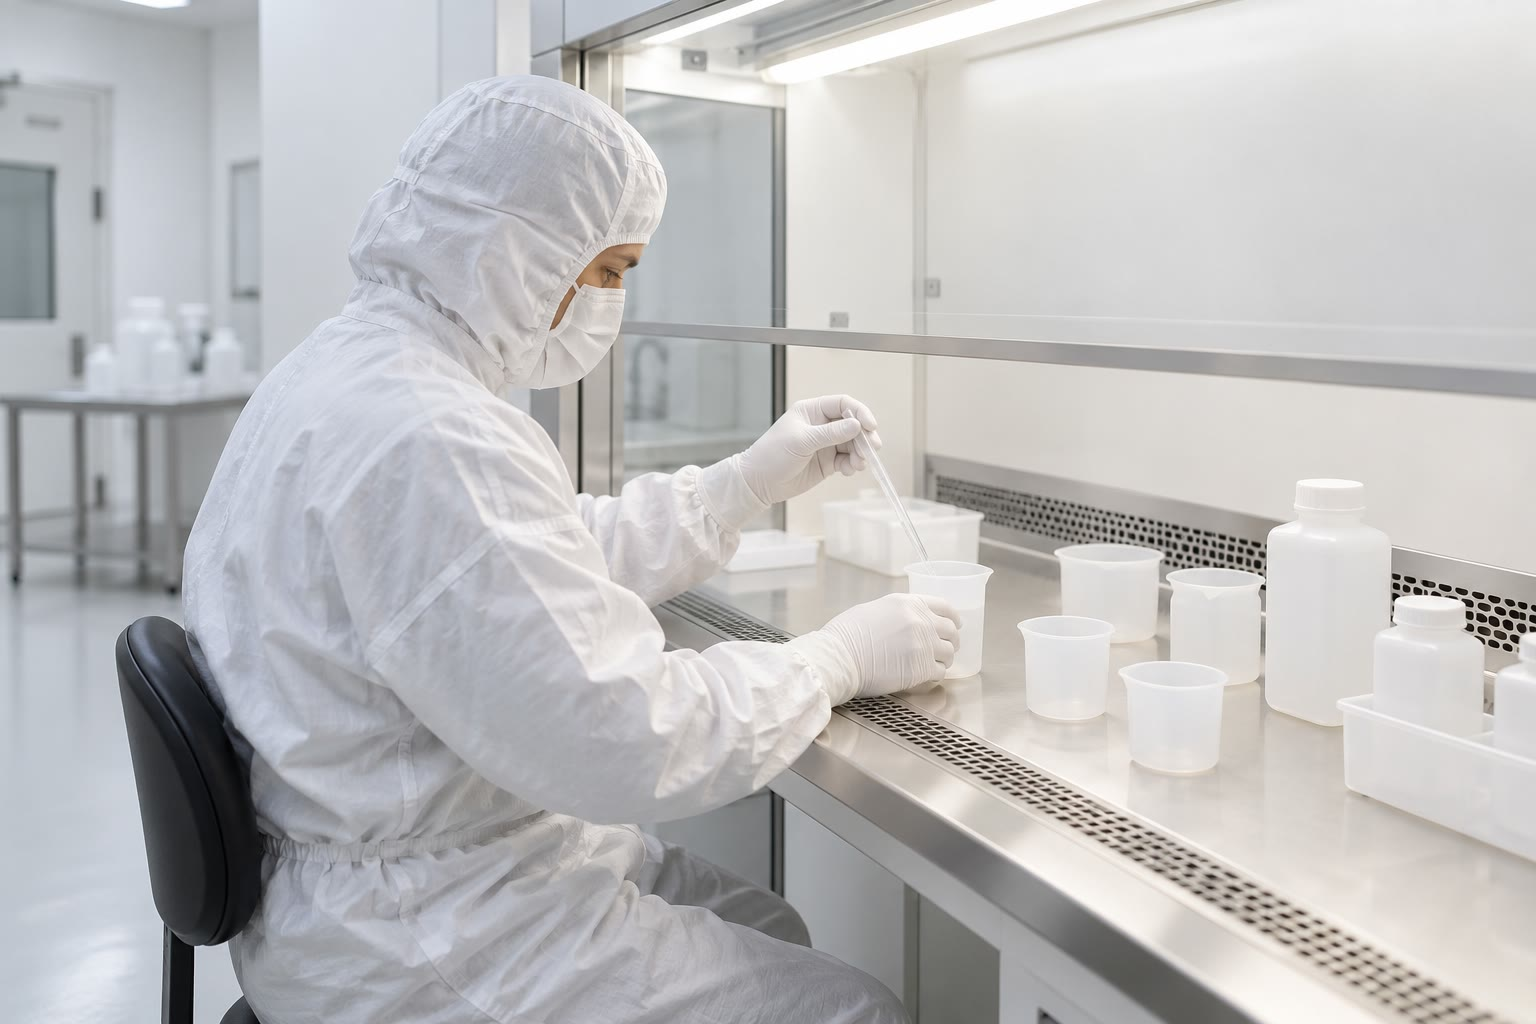
\includegraphics[width=\linewidth]{images/book4/ai/b2-clean-lab.jpg}

\smallskip
{\footnotesize Een medewerker in een cleanroompak aan de laminaire-stromingskast van een
schoon laboratorium voor geochemie (door AI gegenereerde illustratie).\par}
\end{minipage}
\end{inthelab}
% ledger: usgs:bhvo2-trace, usgs:bhvo2-origin

\section{Oefeningen}

\begin{exercise}[$\star$]\label{exo:b2:elements-in-the-earth:1}
Het basalt BHVO-2 bevat 0.5130 procent \ce{K2O} en 2.731 procent \ce{TiO2}
in massa. Bereken met de atoommassa's K 39.10, Ti 47.87 en O 16.00 zijn
kalium- en titaangehalte in ppm.
\end{exercise}

\begin{exercise}[$\star$]\label{exo:b2:elements-in-the-earth:2}
In de \omterm{def:b2:elements-in-the-earth:bse}{totale silicaataarde} zijn de verhoudingen $(X/\mathrm{Mg})$ gedeeld door de CI-verhoudingen
1.16 voor aluminium, 0.22 voor natrium, 0.077 voor nikkel en 0.0029 voor
iridium. De \omterm{def:b2:planet-formation-meteorites:condensation}{condensatietemperaturen} van deze elementen zijn 1653, 958, 1353
en \qty{1603}{K}. Geef de klasse van Goldschmidt van elk element en verklaar elke
verarming.
\end{exercise}

\begin{exercise}[$\star$]\label{exo:b2:elements-in-the-earth:3}
De bovenste continentale korst bevat \qty{31}{ppm} lanthaan en \qty{2.0}{ppm}
ytterbium; \omterm{def:b2:elements-in-the-earth:ci}{CI-chondrieten} 0.232 en \qty{0.163}{ppm}. Bereken de
op \omterm{def:b2:planet-formation-meteorites:chondrule}{chondriet} genormaliseerde waarden en $(\mathrm{La}/\mathrm{Yb})_N$. Wat zegt de
verhouding over de korst?
\end{exercise}

\begin{exercise}[$\star$]\label{exo:b2:elements-in-the-earth:4}
De bovenste continentale korst bevat 4.7, 1.0 en \qty{4.0}{ppm} samarium,
europium en gadolinium; \omterm{def:b2:elements-in-the-earth:ci}{CI-chondrieten} 0.145, 0.0546 en \qty{0.198}{ppm}.
Bereken $\mathrm{Eu}/\mathrm{Eu}^*$. Welk mineraal verklaart het resultaat?
\end{exercise}

\begin{exercise}[$\star\star$]\label{exo:b2:elements-in-the-earth:5}
Een granaatpyroxeniet bestaat uit 65 procent clinopyroxeen, 18 procent granaat en
17 procent olivijn, orthopyroxeen en spinel. De verdelingscoëfficiënten van
lanthaan zijn 0.058, 0.001 en 0.001, die van lutetium 0.53, 5.8 en 0.18.
Bereken de globale coëfficiënten. Welk element is compatibel in het gesteente? Welk
mineraal bevat het grootste deel van het lutetium van het gesteente?
\end{exercise}

\begin{exercise}[$\star\star$]\label{exo:b2:elements-in-the-earth:6}
De \omterm{def:b2:elements-in-the-earth:bse}{totale silicaataarde} bevat 22.8 procent magnesium, \qty{2670}{ppm}
natrium en \qty{1960}{ppm} nikkel; \omterm{def:b2:elements-in-the-earth:ci}{CI-chondrieten} 9.587 procent,
\qty{5010}{ppm} en \qty{10640}{ppm}. Bereken de op Mg genormaliseerde verhoudingen tot CI voor
natrium en nikkel. Beide elementen condenseren rond \qty{1000}{K} of hoger; waarom is
nikkel het sterkst verarmd?
\end{exercise}

\begin{exercise}[$\star\star$]\label{exo:b2:elements-in-the-earth:7}
Een clinopyroxeen kristalliseert uit een smelt met de samenstelling van de gemiddelde MORB,
\qty{5.21}{ppm} lanthaan en \qty{0.53}{ppm} lutetium. Zijn verdelingscoëfficiënten
zijn 0.058 voor lanthaan en 0.53 voor lutetium. Bereken zijn
gehalte aan lanthaan en lutetium, en de verhouding van $(\mathrm{La}/\mathrm{Lu})_N$
in het kristal tot die in de smelt (CI: La 0.232, Lu \qty{0.0237}{ppm}).
\end{exercise}

\begin{exercise}[$\star\star$]\label{exo:b2:elements-in-the-earth:8}
Bereken, genormaliseerd op de \omterm{def:b2:elements-in-the-earth:bse}{primitieve mantel} (Nb \qty{0.658}{ppm}, La \qty{0.648}{ppm}),
$(\mathrm{Nb}/\mathrm{La})_N$ voor de bovenste continentale korst (Nb 12,
La \qty{31}{ppm}), het Hawaïaanse basalt (18.10, \qty{15.20}{ppm}) en de gemiddelde MORB
(5.24, \qty{5.21}{ppm}). Welke ervan draagt het kenmerk van subductiezones?
\end{exercise}

\begin{exercise}[$\star\star$]\label{exo:b2:elements-in-the-earth:9}
Kalium en uranium zijn beide sterk incompatibel. Bereken de massaverhouding K/U in
de \omterm{def:b2:elements-in-the-earth:bse}{primitieve mantel} (K \qty{240}{ppm}, U \qty{0.0203}{ppm}), in de gemiddelde MORB
(\qty{0.160}{\percent} \ce{K2O}, U \qty{0.119}{ppm}) en in de bovenste continentale
korst (\qty{2.80}{\percent} \ce{K2O}, U \qty{2.7}{ppm}), met
$\mathrm{K}/\ce{K2O} = 0.830$ in massa. Wat betekent het feit dat de verhouding bijna constant is,
en waarom is K/U nuttig om het kalium van een planeet te schatten?
\end{exercise}

\begin{exercise}[$\star\star\star$]\label{exo:b2:elements-in-the-earth:10}
Een kleine hoeveelheid smelt is in evenwicht met de granaatpyroxeniet van oefening
5. Toon aan dat voor twee elementen de verhouding
$(C_1/C_2)_{\mathrm{melt}}/(C_1/C_2)_{\mathrm{rock}}$ gelijk is aan
$\bar D_2/\bar D_1$. Bereken ze voor lanthaan en lutetium, en leg uit waarom de
smelten van granaathoudende mantel steile patronen van de \omterm{def:b2:elements-in-the-earth:ree}{zeldzame aarden} hebben.
\end{exercise}

\begin{exercise}[$\star\star\star$]\label{exo:b2:elements-in-the-earth:11}
Een gemiddelde MORB (Th \qty{0.404}{ppm}, Nb \qty{5.24}{ppm}) assimileert bovenste
continentale korst (Th \qty{10.5}{ppm}, Nb \qty{12}{ppm}): een massafractie $f$
korst mengt zich met $1-f$ basalt. Toon aan dat de concentraties van het mengsel
lineair zijn in $f$, maar dat de verhouding Th/Nb dat niet is. Zoek $f$ waarvoor Th/Nb
0.2 bereikt, en de verhouding voor $f = 0.1$.
\end{exercise}

\begin{exercise}[$\star\star\star$]\label{exo:b2:elements-in-the-earth:12}
Het verwijderen van water, koolstof of een metalen kern die aluminium noch
magnesium bevat, verandert de verhouding Al/Mg van de rest niet: toon het aan. In de \omterm{def:b2:elements-in-the-earth:bse}{totale
silicaataarde} is $(\mathrm{Al}/\mathrm{Mg})$ 1.16 keer de CI-waarde. Als de
aarde al haar aluminium heeft behouden, welke fractie van haar chondritische magnesium
ontbreekt dan in de silicaataarde? Welke fractie van haar chondritische silicium zou, met de op Mg
genormaliseerde verhouding van silicium, 0.83, onder dezelfde aanname
ontbreken?
\end{exercise}

\section{Probleem: De kern wegen met een chondriet}

\begin{problem}[{Weekendprobleem --- de aarde als geheel reconstrueren uit CI-chondrieten,
de mantel en de kern, en de kern wegen}]
\label{pb:b2:elements-in-the-earth:1}
Een planetaire geochemicus wil de kern van de aarde wegen zonder seismologie, alleen
met chemie. Ze neemt \omterm{def:b2:elements-in-the-earth:ci}{CI-chondrieten} als uitgangsmateriaal (Mg
\qty{95870}{ppm}, Al 8500, Si \num{106500}, Fe \num{182800}, Ni
\qty{10640}{ppm}), de \omterm{def:b2:elements-in-the-earth:bse}{primitieve mantel} voor de silicaataarde (MgO 37.8, FeO
8.05, NiO 0.25 procent; Mg 22.8, Si 21.0 procent), en een modelkern van 85.5
procent Fe, 5.2 procent Ni en 6.0 procent Si. Atoommassa's: Mg 24.31,
Si 28.09, Fe 55.85, Ni 58.69, O 16.00. Massa van de aarde
\qty{5.972e24}{kg}.

\medskip\noindent\textbf{Deel I --- Het chondritische uitgangspunt.}
\begin{enumerate}
\item Bereken de massaverhoudingen Fe/Mg, Ni/Mg, Si/Mg en Al/Mg van \omterm{def:b2:elements-in-the-earth:ci}{CI-chondrieten}.
\item Reken Fe/Si om naar een atoomverhouding. Spectroscopie van de fotosfeer van de Zon
geeft 0.81 ijzeratoom per siliciumatoom: is de vergelijking zinvol?
\item \omterm{def:b2:elements-in-the-earth:ci}{CI-chondrieten} bevatten 2.1 procent waterstof en 3.5 procent koolstof, gebonden in
waterhoudende mineralen en organische verbindingen die de aarde niet heeft behouden. Waarom
hoeven de verhoudingen van vraag 1 niet voor dit verlies te worden gecorrigeerd?
\item Waarom is magnesium een geschikt referentie-element voor het kernprobleem, en
waarom zou ijzer dat niet kunnen zijn?
\item Nikkel, magnesium, ijzer en silicium condenseren binnen \qty{50}{K} van
elkaar (1353, 1336, 1334 en \qty{1310}{K}). Waarom ondersteunt dit de
aanname dat de aarde als geheel hun chondritische verhoudingen heeft behouden? Welke verhouding van
vraag 1 wijkt van deze groep af, en wat zegt het hoofdstuk erover?
\end{enumerate}

\noindent\textbf{Deel II --- De silicaataarde.}
\begin{enumerate}[resume]
\item Reken het FeO en NiO van de \omterm{def:b2:elements-in-the-earth:bse}{primitieve mantel} om naar Fe en Ni.
\item Bereken Fe/Mg en Ni/Mg in de silicaataarde.
\item Welke fractie van het chondritische Fe en Ni ontbreekt in de silicaataarde,
bij constant magnesium?
\item Dezelfde berekening voor iridium (\omterm{def:b2:elements-in-the-earth:bse}{primitieve mantel} \qty{3.2}{ppb}, CI
\qty{0.470}{ppm}) geeft een ontbrekende fractie van 99.7 procent. Waarom is die groter
dan voor nikkel, en die van nikkel groter dan voor ijzer?
\item Waar zit het ijzer in de silicaataarde, en waarom is het niet allemaal naar de
kern gegaan?
\end{enumerate}

\noindent\textbf{Deel III --- De kern wegen.}
\begin{enumerate}[resume]
\item Schrijf de ijzerbalans van de aarde op met de massafractie $x$ van de kern, en
leid \cref{prop:b2:elements-in-the-earth:core} af.
\item Bereken $y = x/(1-x)$ en $x$ uit het ijzer.
\item Doe hetzelfde met het nikkel.
\item De twee schattingen komen niet precies overeen. Combineer ze met de kleinste kwadraten:
minimaliseer $\sum (a_iy - b_i)^2$, waarbij $a_i y = b_i$ de twee vergelijkingen van de
vragen 12 en 13 zijn, en geef de beste $y$ en $x$.
\item Waarom ligt de kleinste-kwadratenwaarde zo dicht bij de schatting uit het ijzer?
\item Bereken uit de twee vergelijkingen de verhouding Fe/Ni van de kern die
beide exact zou maken. Vergelijk met de modelkern.
\item Geef de massa van de kern.
\end{enumerate}

\noindent\textbf{Deel IV --- Controles en gevolgen.}
\begin{enumerate}[resume]
\item De seismologie geeft een kern van 32.5 procent van de massa van de aarde. Met hoeveel
procent wijkt de chemische schatting af?
\item Hoeveel ijzer zou de kern, met een kern van 32.5 procent, moeten bevatten om
de ijzerbalans te sluiten? Is dit verenigbaar met een kern die voor 10 procent uit lichte
elementen bestaat?
\item De modelkern bevat 9.3 procent andere elementen dan Fe en Ni. Welke
lichte elementen zijn kandidaten, en welk bewijs in het hoofdstuk ondersteunt silicium?
\item Bereken met de $y$ van vraag 14 het siliciumgehalte van de kern dat
de Si/Mg van de aarde als geheel chondritisch zou maken.
\item Vergelijk met de 6 procent van het model. Geef een reden, uit het vorige
hoofdstuk, waarom er misschien wat silicium in de aarde als geheel ontbreekt.
\item De modelkern bevat \qty{0.5}{ppm} goud, de \omterm{def:b2:elements-in-the-earth:bse}{primitieve mantel}
\qty{1}{ppb}. Welke fractie van het goud van de aarde zit, met een kern van 32.5 procent,
in de kern?
\item Geef de massafractie van de kern van de aarde die alleen uit de chemie is verkregen,
het kerngetal van dit probleem.
\end{enumerate}
\end{problem}
% ledger: lodders:ci-table, lodders:ci-h-photo, ms95:pm-oxides, ms95:pm-trace, mcd03:core, earth:mass, badro:core, lodders:tc-table
